\subsection{Obtaining a Toolchain}

\begin{frame}
  \frametitle{Building a toolchain manually}

  \begin{itemize}
  \item Building a cross-compiling toolchain manually is a fairly
    difficult process
  \item Lots of details to learn: many components to build with
    complicated configuration
  \item Typical process is:
    \begin{itemize}
    \item Build dependencies of binutils/gcc (GMP, MPFR, ISL, etc.)
    \item Build {\em binutils}
    \item Build a baremetal, first stage {\em GCC}
    \item Extract kernel headers from the Linux source code
    \item Build the C library using the first stage GCC
    \item Build the second stage and final {\em GCC} supporting the Linux
          OS and the C library.
    \end{itemize}
  \item Many decisions to make about the components: C library, gcc
    and binutils versions, ABI, floating point mechanisms, etc. Not
    trivial to find correct combinations of these possibilities
  \item See the
    \href{https://crosstool-ng.github.io/docs/toolchain-construction/}{Crosstool-NG
      documentation} for details on how toolchains are built.
  \item Talk: {\em Anatomy of Cross-Compilation Toolchains}, by Thomas
    Petazzoni, ELCE 2017, \href{https://youtu.be/Pbt330zuNPc}{video} and
    \href{https://elinux.org/images/1/15/Anatomy_of_Cross-Compilation_Toolchains.pdf}{slides}
\end{itemize}
\end{frame}

\begin{frame}
  \frametitle{Get a pre-compiled toolchain}
  \begin{itemize}
  \item Solution that many people choose
    \begin{itemize}
    \item Advantage: it is the simplest and most convenient solution
    \item Drawback: you can't fine tune the toolchain to your needs
    \end{itemize}
  \item Make sure the toolchain you find meets your requirements: CPU,
    endianness, C library, component versions, version of the kernel
    headers, ABI, soft float or hard float, etc.
  \item Some possibilities:
    \begin{itemize}
    \item Toolchains packaged by your distribution, for example Ubuntu
      package
      \href{https://packages.ubuntu.com/gcc-arm-linux-gnueabihf}{gcc-arm-linux-gnueabihf}
      or Fedora
      \href{https://packages.fedoraproject.org/pkgs/cross-gcc/gcc-arm-linux-gnu/}{gcc-arm-linux-gnu}. Often
      limited to ARM/ARM64 with glibc.
    \item Bootlin's GNU toolchains, most CPU architectures, with
      glibc/uClibc/musl, \url{https://toolchains.bootlin.com}
    \item \href{https://developer.arm.com/tools-and-software/open-source-software/developer-tools/gnu-toolchain/downloads}
      {ARM and ARM64 toolchains released by ARM}
    \end{itemize}
  \end{itemize}
\end{frame}

\begin{frame}{Example of toolchains from ARM: downloading}
  \begin{columns}
    \column{0.6\textwidth}
    \begin{center}
      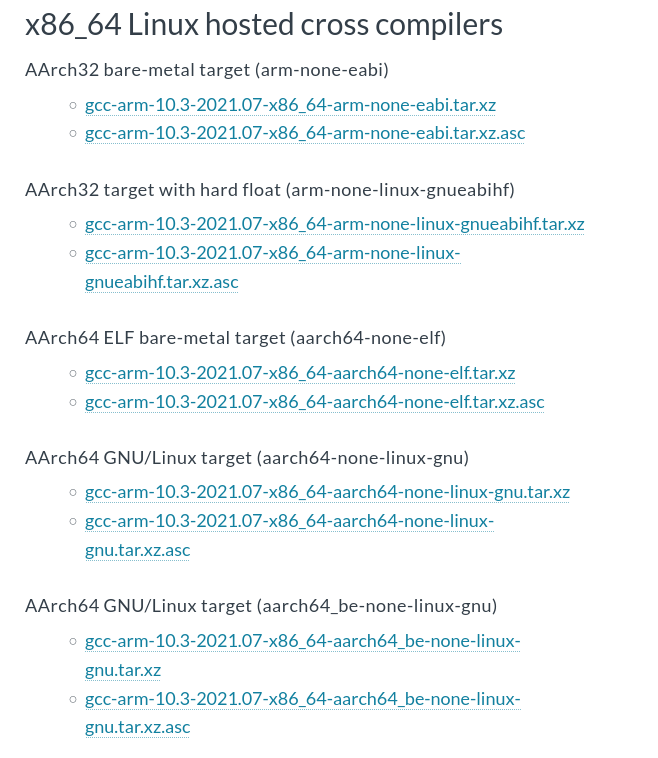
\includegraphics[height=0.8\textheight]{slides/linux-toolchains-obtaining/arm-toolchain.png}
    \end{center}
    \column{0.4\textwidth}
    From \href{https://developer.arm.com/tools-and-software/open-source-software/developer-tools/gnu-toolchain/downloads}
    {Arm GNU Toolchains}
  \end{columns}
\end{frame}

\begin{frame}[fragile]{Example of toolchains from ARM: using}
  \begin{block}{}
    {\tiny
\begin{verbatim}
$ wget https://developer.arm.com/-/media/Files/downloads/gnu-a/10.3-2021.07/binrel/[...]
    [...]gcc-arm-10.3-2021.07-x86_64-arm-none-linux-gnueabihf.tar.xz

$ tar xf gcc-arm-10.3-2021.07-x86_64-arm-none-linux-gnueabihf.tar.xz

$ cd gcc-arm-10.3-2021.07-x86_64-arm-none-linux-gnueabihf/

$ ./bin/arm-none-linux-gnueabihf-gcc -o test test.c

$ file test
test: ELF 32-bit LSB executable, ARM, EABI5 version 1 (SYSV), dynamically linked, interpreter /lib/ld-linux-armhf.so.3, [...]
   for GNU/Linux 3.2.0, with debug_info, not stripped
\end{verbatim}
    }
  \end{block}
\end{frame}

\begin{frame}
  \frametitle{Toolchain building utilities}
  Another solution is to use utilities that {\bf automate the process of
  building the toolchain}
  \begin{itemize}
  \item Same advantage as the pre-compiled toolchains: you don't need
    to mess up with all the details of the build process
  \item But also offers more flexibility in terms of toolchain
    configuration, component version selection, etc.
  \item Allows to rebuild the toolchain if needed to fix a bug or
    security issue.
  \item They also usually contain several patches that fix known
    issues with the different components on some architectures
  \item Multiple tools with identical principle: shell scripts or
    Makefile that automatically fetch, extract, configure, compile and
    install the different components
\end{itemize}
\end{frame}

\begin{frame}
  \frametitle{Toolchain building utilities (2)}
  \begin{columns}
  \column{0.6\textwidth}
    {\bf Crosstool-ng}
    \begin{itemize}
      \item Rewrite of the older Crosstool, with a menuconfig-like configuration
	system
      \item Feature-full: supports uClibc, glibc and musl,
            hard and soft float, many architectures
      \item Actively maintained
      \item \url{https://crosstool-ng.github.io/}
    \end{itemize}
  \column{0.4\textwidth}
    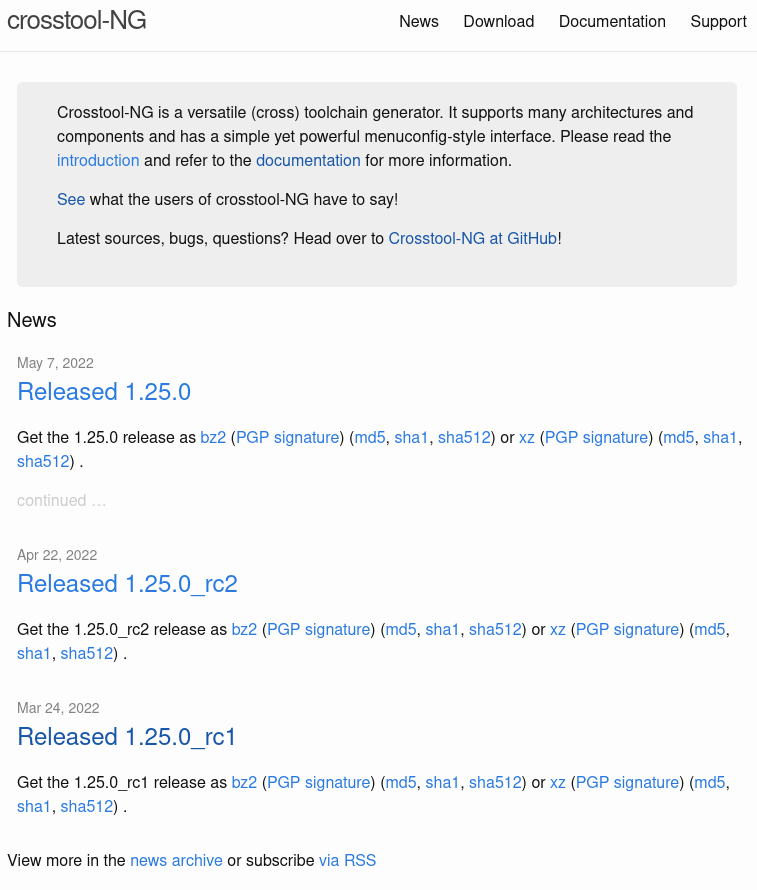
\includegraphics[width=\textwidth]{slides/linux-toolchains-obtaining/crosstool-ng.png}
  \end{columns}
\end{frame}

\begin{frame}
\frametitle{Toolchain building utilities (3)}
Many root filesystem build systems also allow the construction of
a cross-compiling toolchain
\begin{itemize}
\item {\bf Buildroot}
  \begin{itemize}
  \item Makefile-based. Can build glibc, uClibc and musl based
    toolchains, for a wide range of architectures. Use \code{make sdk}
    to only generate a toolchain.
  \item \url{https://buildroot.org}
  \end{itemize}
\item {\bf PTXdist}
  \begin{itemize}
  \item Makefile-based, maintained mainly by {\em Pengutronix},
        supporting only glibc and uClibc (version 2023.01 status)
  \item \url{https://www.ptxdist.org/}
  \end{itemize}
\item {\bf OpenEmbedded / Yocto Project}
  \begin{itemize}
  \item A featureful, but more complicated build system, supporting only
        glibc and musl.
  \item \url{https://www.openembedded.org/}
  \item \url{https://www.yoctoproject.org/}
  \end{itemize}
\end{itemize}
\end{frame}

\begin{frame}[fragile]{Crosstool-NG: download}
  \begin{itemize}
  \item Getting Crosstool-NG
\begin{verbatim}
$ git clone https://github.com/crosstool-ng/crosstool-ng.git
\end{verbatim}
  \item Using a well-known stable version
\begin{verbatim}
$ cd crosstool-ng
$ git checkout crosstool-ng-1.27.0
\end{verbatim}
  \item As we're fetching from Git, the \code{configure} script needs
    to be generated:
\begin{verbatim}
$ ./bootstrap
\end{verbatim}
  \end{itemize}
\end{frame}

\begin{frame}[fragile]{Crosstool-NG: installation}
  \begin{itemize}
  \item Installation can be done:
    \begin{itemize}
    \item system-wide, for example in \code{/usr/local}, the
      \code{ct-ng} command is then available globally
\begin{verbatim}
$ ./configure
$ make
$ sudo make install
\end{verbatim}
    \item or just locally in the source directory, the \code{ct-ng}
      command will be invoked from this directory
\begin{verbatim}
$ ./configure --enable-local
$ make
\end{verbatim}
    \end{itemize}
  \item Note: the \code{make} invocation doesn't build any toolchain,
    it builds the \code{ct-ng} executable.
  \end{itemize}
\end{frame}

\begin{frame}{Crosstool-NG: toolchain configuration}
  \begin{itemize}
  \item Once installed, the \code{ct-ng} tool allows to configure and
    build an arbitrary number of toolchains
  \item Its configuration system is based on {\em kconfig}, like the
    Linux kernel configuration system
  \item Configuration of the toolchain to build stored in a
    \code{.config} file
  \item Example configurations provided with Crosstool-NG
    \begin{itemize}
    \item List: \code{./ct-ng list-samples}
    \item Load an example: \code{./ct-ng <sample-name>}, replaces \code{.config}
    \item For example \code{./ct-ng aarch64-unknown-linux-gnu}
    \item No sample loaded
      $\rightarrow$ default Crosstool-NG configuration is a bare-metal
      toolchain for the {\em Alpha} CPU architecture!
    \end{itemize}
  \item The configuration can then be refined using either:
    \begin{itemize}
    \item \code{./ct-ng menuconfig}
    \item \code{./ct-ng nconfig}
    \end{itemize}
  \end{itemize}
\end{frame}

\begin{frame}{Crosstool-NG: toolchain configuration}
  \begin{center}
    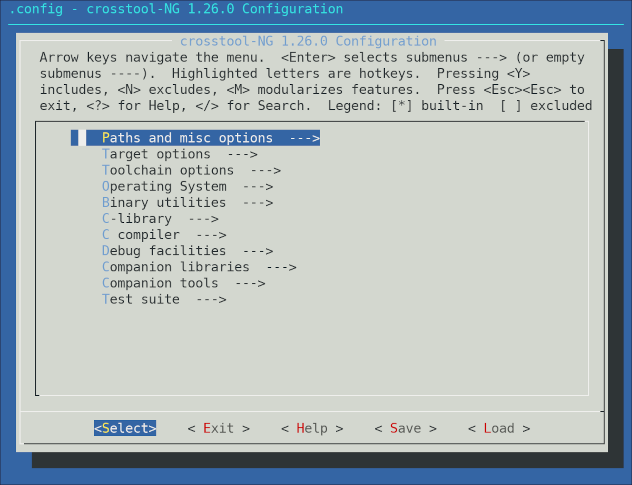
\includegraphics[height=0.7\textheight]{slides/linux-toolchains-obtaining/ct-ng-menu.png}
    \vspace{0.1cm}\\
    \code{./ct-ng menuconfig}
  \end{center}
\end{frame}

\begin{frame}[fragile]{Crosstool-NG: toolchain building}
  \begin{itemize}
  \item To build the toolchain
\begin{verbatim}
./ct-ng build
\end{verbatim}
    This will automatically download all the needed dependencies, and
    build all toolchain components in the right order, with the
    specified configuration.
  \item By default the results go in
    \code{$HOME/x-tools/<architecture-tuple>}, as defined by the
    option \code{CT_PREFIX_DIR} in {\em Paths and misc options}
  \end{itemize}
\end{frame}

\begin{frame}[fragile]{Important toolchain contents}
  \begin{itemize}
  \item \code{bin/}: cross compilation tool binaries
    \begin{itemize}
    \item This directory can be added to your \code{PATH} to ease
      usage of the toolchain
    \item Sometimes with symlinks for shorter names
\begin{verbatim}
arm-linux-gcc -> arm-cortexa7-linux-uclibcgnueabihf-gcc
\end{verbatim}
    \end{itemize}
  \item \code{<arch-tuple>/sysroot}: {\em sysroot} directory
    \begin{itemize}
    \item \code{<arch-tuple>/sysroot/lib}: C library, GCC runtime, C++
      standard library compiled for the target
    \item \code{<arch-tuple>/sysroot/usr/include}: C library headers
      and kernel headers
    \end{itemize}
  \end{itemize}
\end{frame}
